\section{Anwendungen und Beispiele}

\subsection{Klangwiedergange einer Geige}

\begin{frame}
  \frametitle{Klangcharakteristika einer Geige}
  \begin{figure}
    \centering
    \only<1>{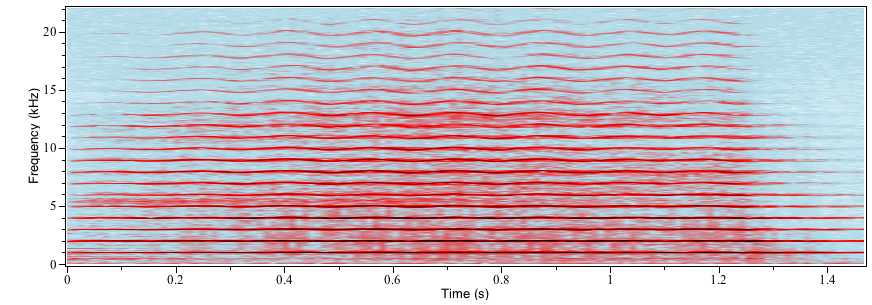
\includegraphics[width=\linewidth]{img/violin}}
    \only<2>{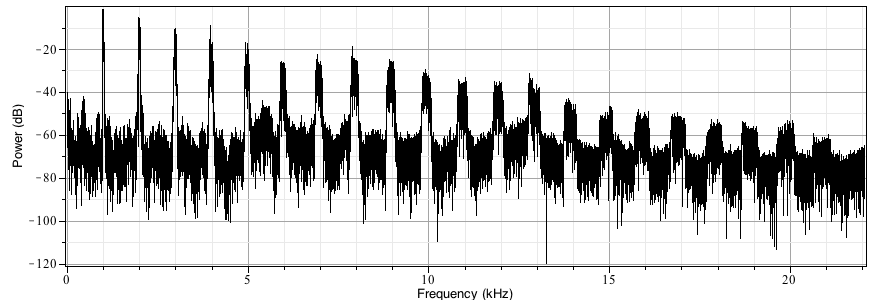
\includegraphics[width=\linewidth]{img/violin_power}}
    \label{img:violin}
  \end{figure}
\end{frame}

\subsection{Charakteristika von Sprache}

\begin{frame}
  \frametitle{Sprache}
    \begin{figure}
      \centering
      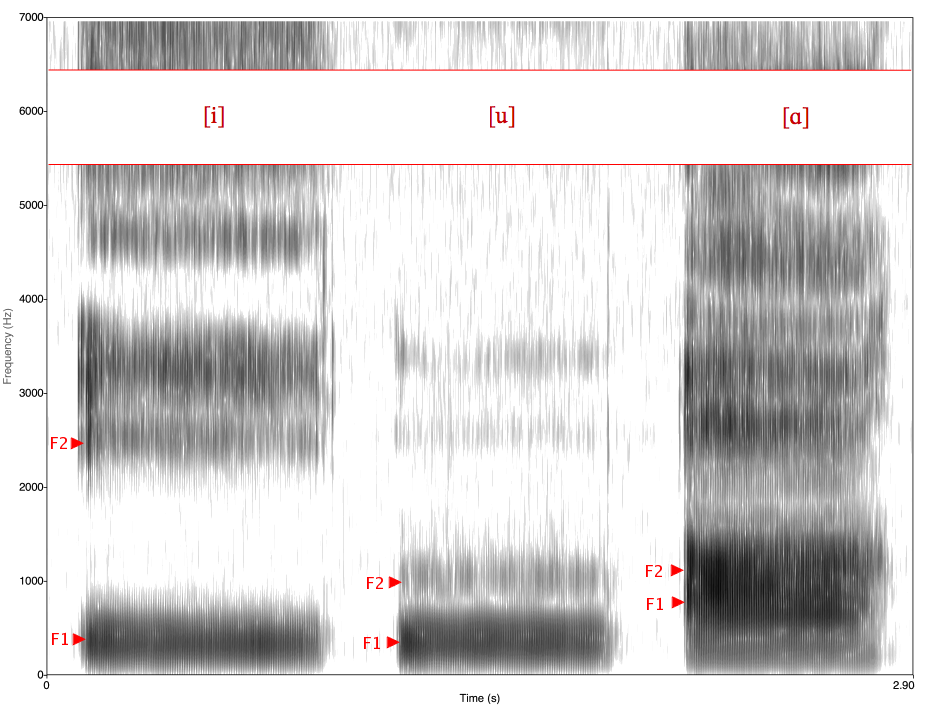
\includegraphics[width=0.8\linewidth]{img/iua}
      \label{img:vowls}
      \caption{\url{https://commons.wikimedia.org/wiki/File:Spectrogram_-iua-.png}, 02.12.15}
    \end{figure}
\end{frame}

\begin{frame}
  \frametitle{Sprache}
    \begin{figure}
      \centering
      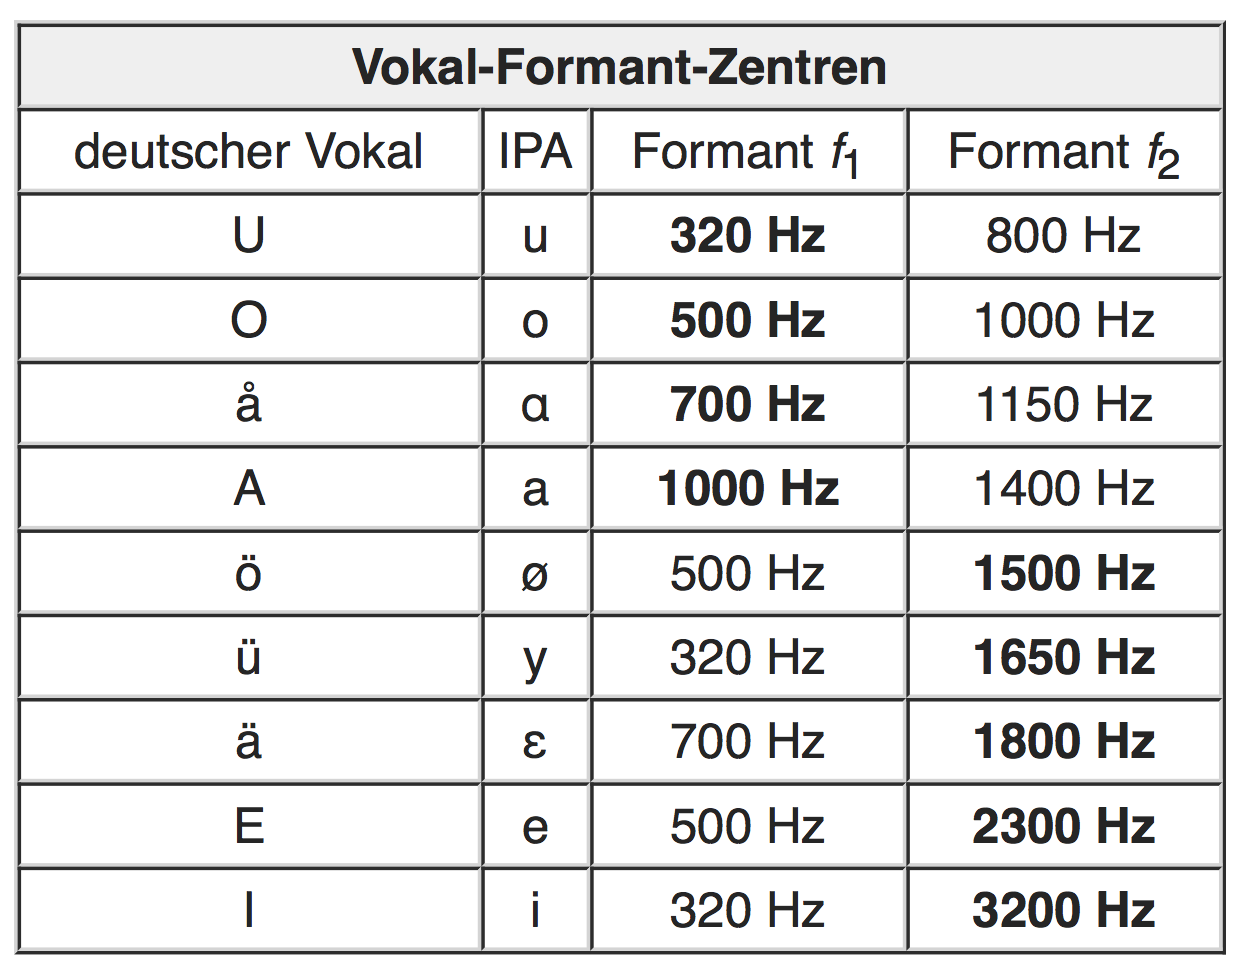
\includegraphics[width=0.8\linewidth]{img/formanten}
      \label{img:vowls}
    \end{figure}
\end{frame}
